%%% Template originaly created by Karol Kozioł (mail@karol-koziol.net) and modified for ShareLaTeX use

\documentclass[a4paper,11pt]{article}

\usepackage[T1]{fontenc}
\usepackage[utf8]{inputenc}
\usepackage{graphicx}
\usepackage{xcolor}

\renewcommand\familydefault{\sfdefault}
\usepackage{tgheros}
\usepackage[defaultmono]{droidmono}

\usepackage{amsmath,amssymb,amsthm,textcomp}
\usepackage{enumerate}
\usepackage{multicol}
\usepackage{tikz}

\usepackage{geometry}
\geometry{total={210mm,297mm},
left=25mm,right=25mm,%
bindingoffset=0mm, top=20mm,bottom=20mm}


\linespread{1.3}

\newcommand{\linia}{\rule{\linewidth}{0.5pt}}

% custom theorems if needed
\newtheoremstyle{mytheor}
    {1ex}{1ex}{\normalfont}{0pt}{\scshape}{.}{1ex}
    {{\thmname{#1 }}{\thmnumber{#2}}{\thmnote{ (#3)}}}

\theoremstyle{mytheor}
\newtheorem{defi}{Definition}

% my own titles
\makeatletter
\renewcommand{\maketitle}{
\begin{center}
\vspace{2ex}
{\huge \textsc{\@title}}
\vspace{1ex}
\\
\linia\\
\@author \hfill \@date
\vspace{4ex}
\end{center}
}
\makeatother
%%%

% custom footers and headers
\usepackage{fancyhdr}
\pagestyle{fancy}
\lhead{}
\chead{}
\rhead{}
\lfoot{Tarea chica 1}
\cfoot{}
\rfoot{Página \thepage}
\renewcommand{\headrulewidth}{0pt}
\renewcommand{\footrulewidth}{0pt}
%

% code listing settings
\usepackage{listings}
\lstset{
    basicstyle=\ttfamily\small,
    aboveskip={1.0\baselineskip},
    belowskip={1.0\baselineskip},
    columns=fixed,
    extendedchars=true,
    breaklines=true,
    tabsize=4,
    prebreak=\raisebox{0ex}[0ex][0ex]{\ensuremath{\hookleftarrow}},
    frame=lines,
    showtabs=false,
    showspaces=false,
    showstringspaces=false,
    keywordstyle=\color[rgb]{0.627,0.126,0.941},
    commentstyle=\color[rgb]{0.133,0.545,0.133},
    stringstyle=\color[rgb]{01,0,0},
    numbers=left,
    numberstyle=\small,
    stepnumber=1,
    numbersep=10pt,
    captionpos=t,
    escapeinside={\%*}{*)}
}

%%%----------%%%----------%%%----------%%%----------%%%

\begin{document}

\title{Tarea chica 1\\Sistema Operativo: Command Line}

\author{Diego Andai Castilla, Universidad Católica de Chile}

\date{17/04/2016}

\maketitle

\section{Codecademy.com}

Imagen que acredita la aprobaci\'on del curso:

\begin{center}
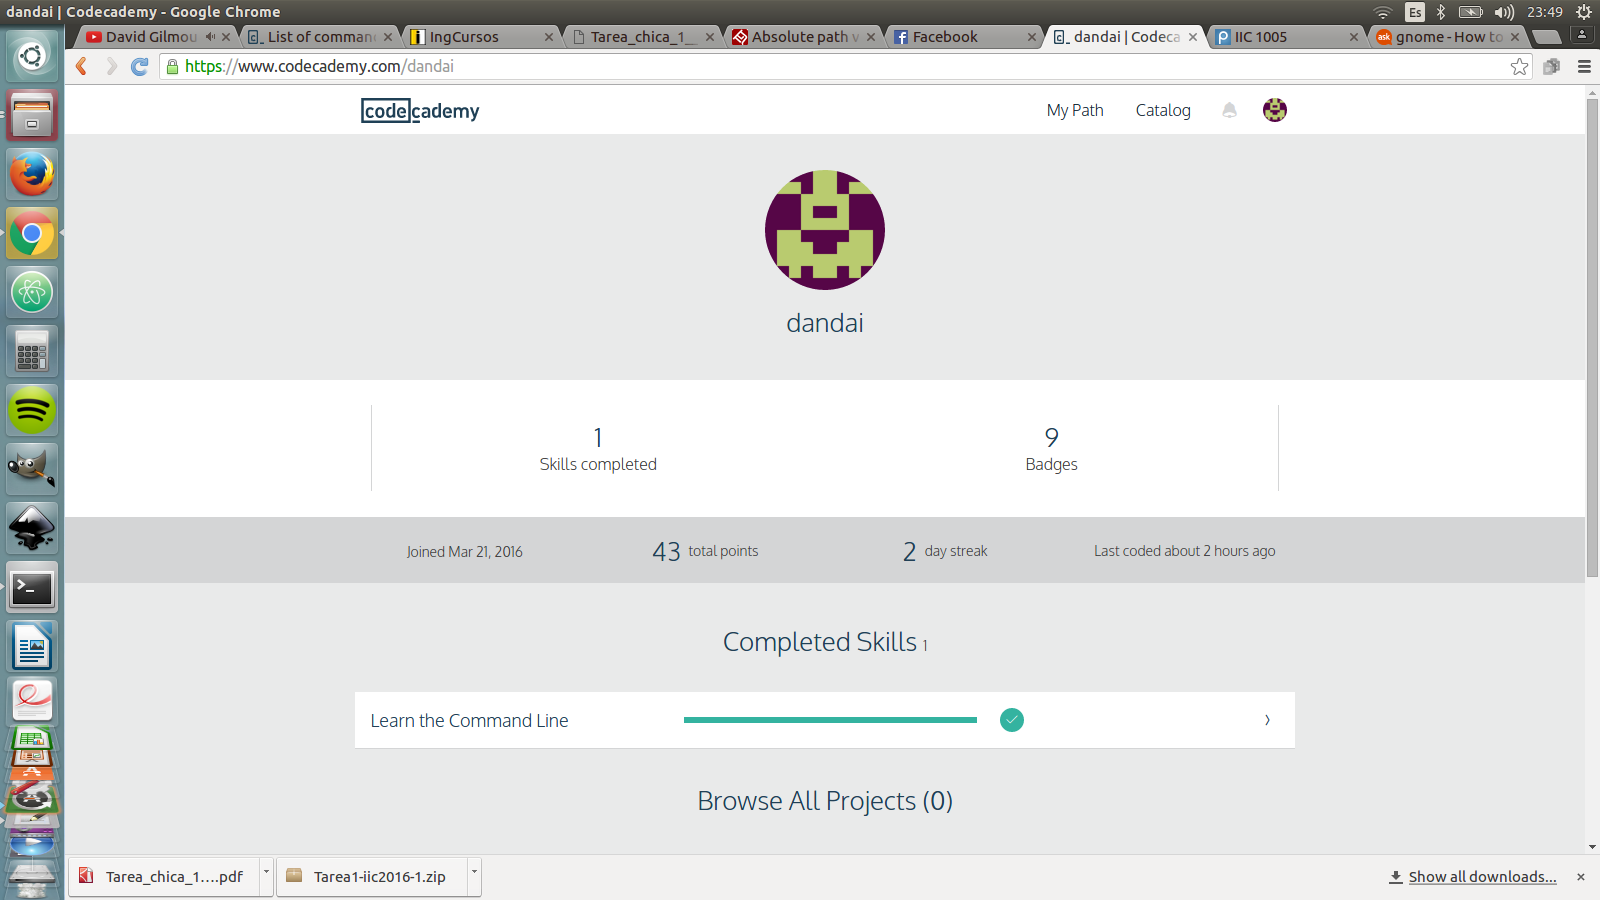
\includegraphics[scale=0.25]{codecademytc1.png}
\end{center}

\section{Manipulación de archivos}

A continuación se resuelven e implementan los diez pasos que constituyen la tarea. Primero se descargó el archivo 20newsgroups.tar.gz del Siding, a la carpeta Downloads.

\subsection{Descomprimir el archivo}

Para el primer paso de la tarea se pide descomprimir el archivo, para esto se ocupa el siguiente comando:

\begin{lstlisting}
gzip -d < 20newsgropus.tar.gz | tar xvf -
\end{lstlisting}

Ya que el archivo tiene extensión \textit{.tar.gz}, hay que ocupar dos comandos, que se implementan en una linea. Al comando \textbf{gzip}, para la extensión \textit{.gz}, se le entrega el archivo con el símbolo '<'. Luego se conecta este comando mediante '|'  a \textbf{tar xvf -}, ocupado para la extensión \textit{.tar}. Esto último se llama \textit{pipe}, nombre que simboliza una comunicación entre comandos.\\

A continuación se muestran imágenes de la implementación.
\begin{center}
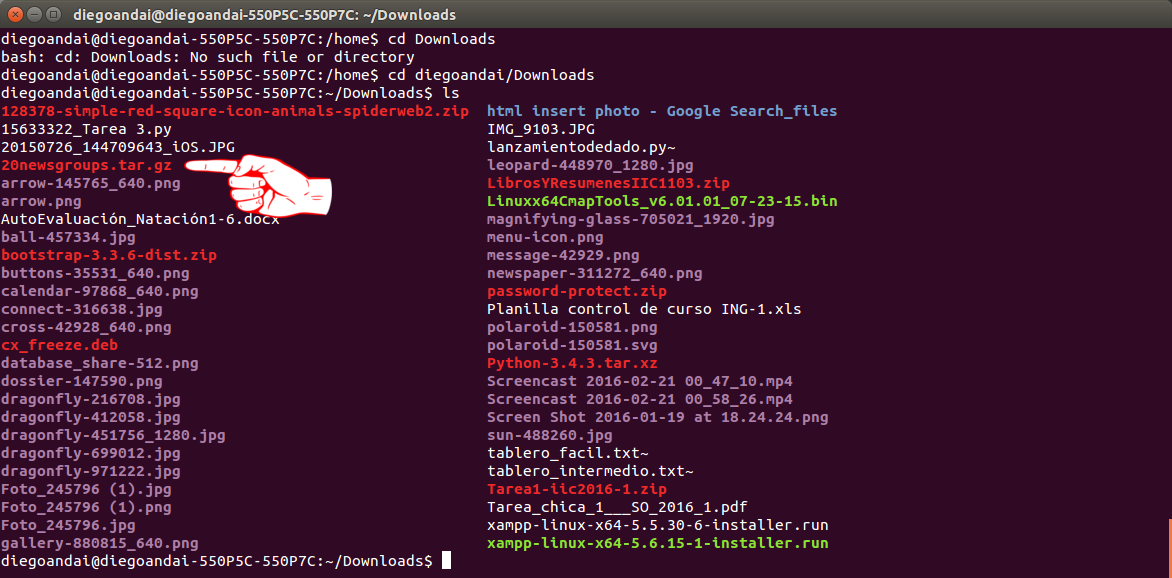
\includegraphics[scale=0.385]{tc1_2.png}
\end{center}
En la imagen anterior se puede ver el archivo descargado, indicado con el símbolo (
\includegraphics[scale=0.03]{finger.png}), 20newsgroups.tar.gz, que se encuentra en la carpeta Downloads.

\begin{center}
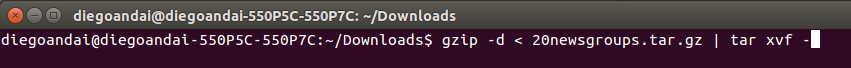
\includegraphics[scale=0.53]{tc1_3.png}
\end{center}

Este es el comando descrito anteriormente, para descomprimir el archivo.

\begin{center}
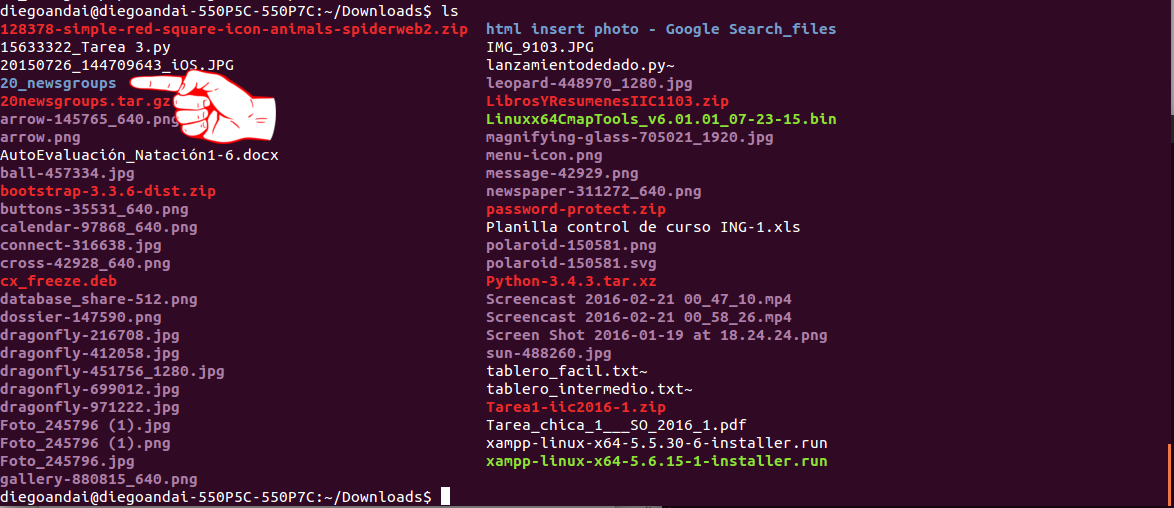
\includegraphics[scale=0.385]{tc1_4.png}
\end{center}

Como se puede apreciar despues de la implementación del comando, se ha creado una carpeta de los archivos descomprimidos, con el nombre 20\_newsgroups. Esta carpeta se encuentra aún en Downloads.

\subsection{Mover la carpeta al escritorio}

Para esta tarea se ocupará el comando \textbf{mv}:

\begin{lstlisting}
mv [nombre del directorio o archivo a mover] [directorio de destino]
\end{lstlisting}

Por lo tanto en este caso es:

\begin{lstlisting}
mv 20_newsgroups/ /home/diegoandai/Desktop/
\end{lstlisting}

\begin{center}
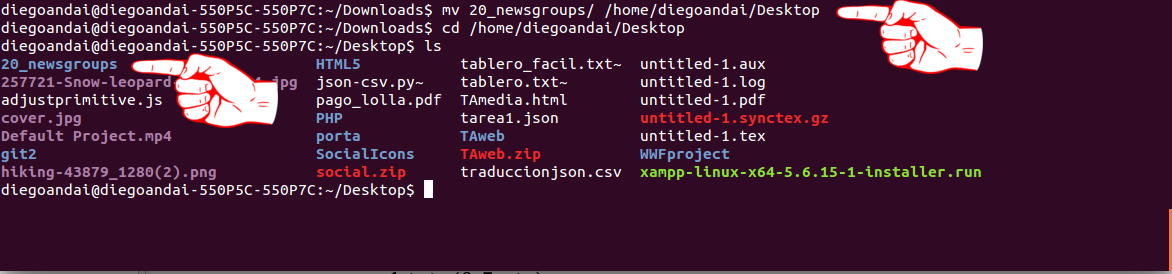
\includegraphics[scale=0.385]{tc1_5.png}
\end{center}

En esta imagen se muestra la implementación de lo anterior. La primera indicación muestra el uso de comando. Se dirige luego al escritorio y se ocupa el comando \textbf{ls}, para mostrar los archivos que en este directorio se encuentran. Efectivamente comprobamos que, en la segunda indicación, podemos ver el directorio que se movió.

\subsection{Cambiar el nombre del directorio}

Para este cometido también se ocupa el comando \textbf{mv}, que tiene esta doble función, ahora lo ocupamos de la siguiente manera:

\begin{lstlisting}
mv [nombre del directorio o archivo con el nombre original] [nuevo nombre]
\end{lstlisting}

Por lo tanto en este caso es:

\begin{lstlisting}
mv 20_newsgroups/ TareaChica1/
\end{lstlisting}

\begin{center}
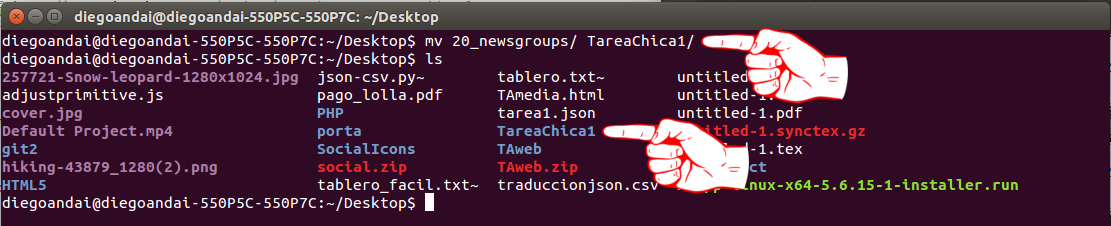
\includegraphics[scale=0.41]{tc_paso3.png}
\end{center}

En la imagen anterior se puede ver el comando siendo utilizado, en la primera indicación. luego se ve que el nombre del drectorio cambió. Nótese que ya no hay ningun directorio llamado 20\_newsgroups, y apareció en cambio TareaChica1.

\subsection{Crear un directorio en TareaChica1}

Se procede a crear un directorio llamado NombreApellido\footnote{Este no es el nombre correcto que estipulaba la tarea, debió haber sido DiegoAndai. Esto se corrige más adelante.}. para esto se ocupa el comando \textbf{mkdir}:

\begin{lstlisting}
mkdir [nombre del nuevo directorio]
\end{lstlisting}

Por lo que en este caso sería:

\begin{lstlisting}
mkdir NombreApellido
\end{lstlisting}

\begin{center}
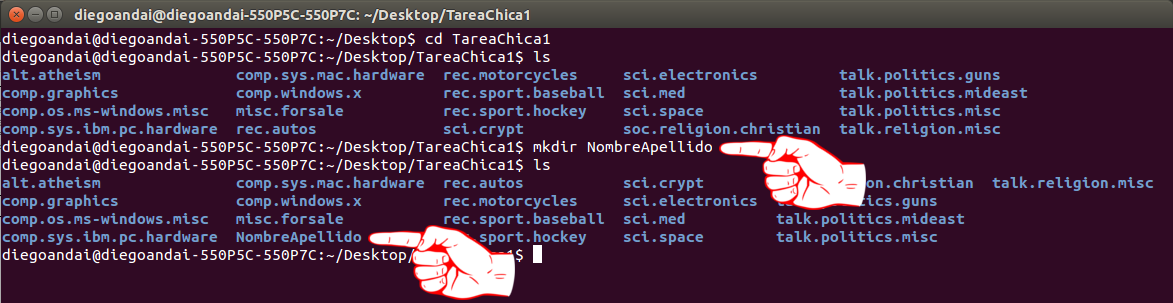
\includegraphics[scale=0.385]{tc1_6.png}
\end{center}

En esta captura de imagen se ven primero los contenidos de TareaChica1. Luego se indica la implementación del comando. Por último se indica el directorio creado, nótese que antes esta no existía.

\subsection{Crear archivos en NombreApellido}

Ahora se crearán dos archivos, p1.txt y p2.txt en el directorio NombreApellido, para esto se ocupará el comando \textbf{touch}:

\begin{lstlisting}
touch [nombre del nuevo archivo]
\end{lstlisting}

Por lo que en este caso sería:

\begin{lstlisting}
touch p1.txt
touch p2.txt
\end{lstlisting}

\begin{center}
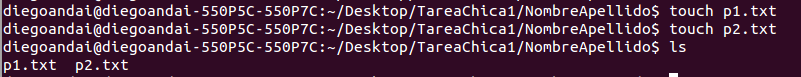
\includegraphics[scale=0.55]{tc1_7.png}
\end{center}

Se puede ver en la imagen anterior la implementación de los comandos. Luego se revisa el directorio, viendo que efectivamente se crearon ambos archivos.

\subsection{Mover contenidos entre carpetas}

Ahora se moverán múltiples archivos de un directorio a otra, específicamente, se moverán todos los archivos en comp.graphics a comp.os.ms-windows.misc (Ambos ubicados en TareaChica1). Para esto ocuparemos el comando \textbf{mv}:

\begin{lstlisting}
mv [nombre del directorio o archivo a mover] [directorio de destino]
\end{lstlisting}

Además, ocuparemos el símbolo '*', denominado \textit{wildcard}. Este representa \textit{cualquier cosa}, con esto me refiero a que si, por ejemplo, ocupo el comando \textit{mv} y como archivo a mover introduzco *.txt, todos los archivos que terminan en .txt se moveran. Para completar la tarea entonces ocupamos:

\begin{lstlisting}
mv comp.graphics/* comp.os.ms-windows.misc/
\end{lstlisting}

\begin{center}

\includegraphics[scale=0.47]{tc1_9.png}
\end{center}

Aquí se ve la implementación del comando. Este envía todos los archivos que tienen el prefijo \textbf{comp.graphics/}, es decir, todos los que pertenecen a ese directorio.

En las siguientes imágenes se puede ver como el directorio tenía archivos que después no están:

\begin{center}
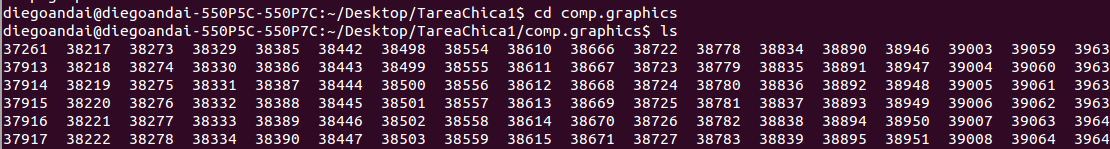
\includegraphics[scale=0.4]{tc1_8.png}
\end{center}

\begin{center}

\includegraphics[scale=0.4]{tc1_9(2).png}
\end{center}

\subsection{Crear contenidos en p2.txt}

A continuación se escribirá en el archivo p2.txt, específicamente, se escribirán en él todos los archivos en TareaChica1 que, dentro de sí, contengan la palabra \textit{terminal}. Para esto se ocuparán los comandos \textbf{grep}, \textbf{sort} y \textbf{uniq}:

El comando \textbf{grep} busca contenidos determinados en los archivos del directorio en que está (también se le puede indicar el directorio en el que tiene que buscar), acepta modos como que retorne sólo el path de donde encontró el string. El comando \textbf{sort} sirve para ordenar alfabéticamente una lista. El comando \textbf{uniq} elimina los elementos adyacentes de una lista que son idénticos:

\begin{lstlisting}
grep [modo] [string por buscar] [directorio en el cual buscar]
sort [lista]
uniq [lista]
\end{lstlisting}

\begin{center}
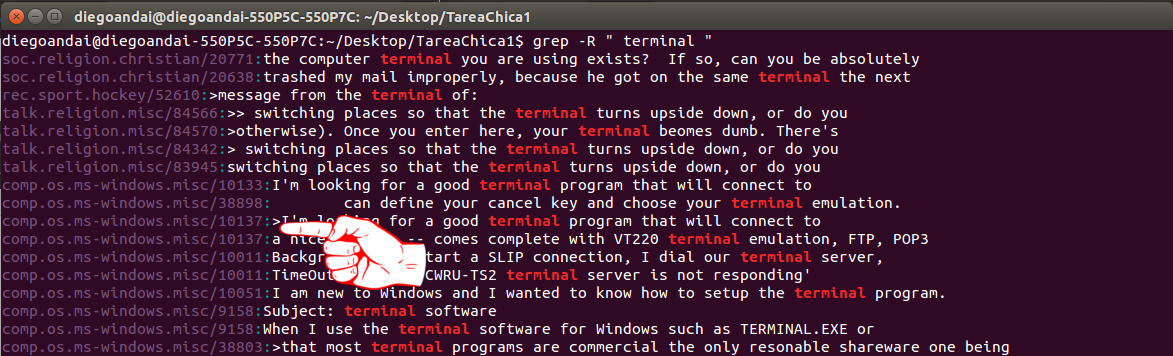
\includegraphics[scale=0.385]{tc1_10.png}
\end{center}

En la imagen anterior se puede ver el output de \textbf{grep}, en este se muestra el path y la frase en que se encontró la palabra. Note tres cosas:

\begin{enumerate}
    \item al archivo p2.txt solo hay que escribir el path, por lo tanto se necesita una forma de aislarlo.
    \item los items no están en orden.
    \item en el lugar que se indica, hay un path repetido, ese no debiera agregarse archivo.
\end{enumerate}

Para poder redirigir los paths obtenidos, estos tres comandos se concatenan mediante \textit{pipes} ('|'):

\begin{lstlisting}
grep -Rl " terminal " | sort | uniq > NombreApellido/p2.txt
\end{lstlisting}

Esto funciona de la siguiente manera:
\begin{enumerate}
    \item grep busca la palabra \textit{terminal} en el directorio en el que se ejecuta. El modo -Rl refiere a que haga una búsqueda recursiva (-R), o sea que busque por todas las carpetas, además hace que retorne solo el path (-l) y no el contenido donde se encontró la palabra.
    \item mediante el \textit{pipe} grep le "pasa" su output a sort, este lo ordena y se lo "pasa" a uniq, que elimina posibles repeticiones. Es importante que antes se hayan ordenado los datos, así los archivos iguales quedaran adyacentes y uniq los eliminará efectivamente.
    \item para finalizar, se ocupa el símbolo '>' para escribir el resultado del lado izquierdo en el archivo, que tiene el path  NombreApellido/p2.txt.
\end{enumerate}

\begin{center}
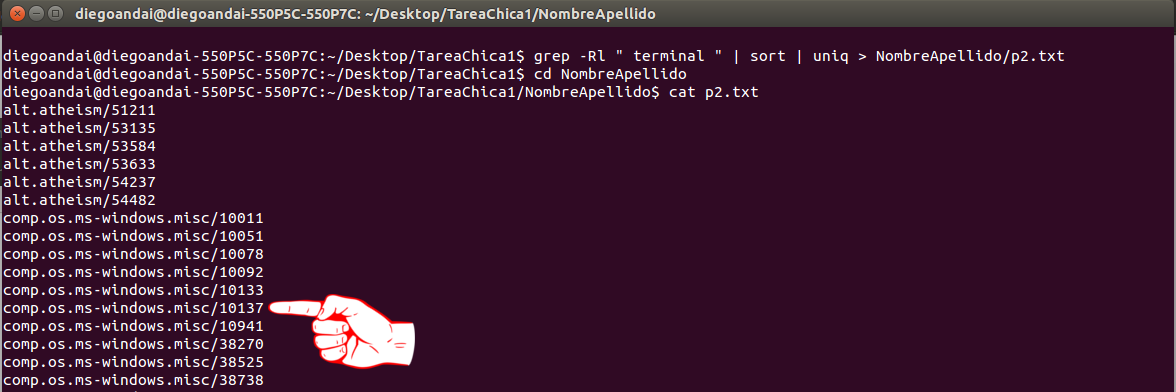
\includegraphics[scale=0.385]{tc1_11.png}
\end{center}

En la imagen anterior, se ve la implementación del comando y luego, con el comando \textbf{cat} se muestra lo que el archivo contiene. Nótese la indicación, el archivo que antes estaba repetido no se agregó dos veces.

\subsection{Copiar contenido de archivos}

Para el siguiente paso, se copia un archivo específico a p1.txt. El archivo que estamos buscando está en el directorio talk.politics.guns y contiene el string \textit{1 out of three}. Para lo anterior ocuparemos el comando \textbf{grep} y el comando para copiar, \textbf{cp}:

\begin{lstlisting}
grep [modo] [string por buscar] [directorio en el cual buscar]
cp [Archivo que se va a copiar] [Adonde se va a copiar]
\end{lstlisting}

Para este caso sería:

\begin{lstlisting}
grep -R "1 out of three" talk.politics.guns/
\end{lstlisting}

\begin{center}
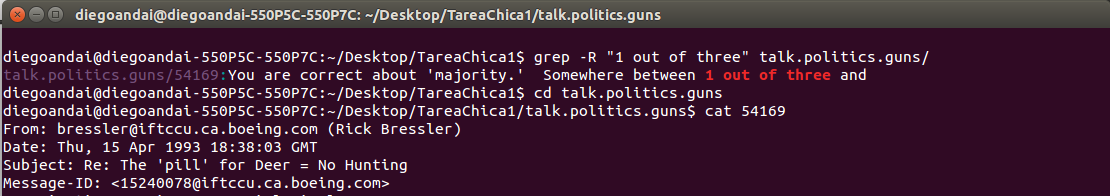
\includegraphics[scale=0.4]{tc1_paso8.png}
\end{center}

Luego de ejecutar el comando en la imagen anterior, sabemos el archivo que necesitamos copiar (54196).Se muestran los contenidos de dicho archivo con el comando \textbf{cat}. Note la última línea, en la que se muestra el ID de la conversación, después se comparará con el ID copiado a p1.txt.

Para copiar hacemos lo siguiente (encontrándonos en el directoriotalk.politics.guns) :

\begin{lstlisting}
cp 5419 ../NombreApellido/p1.txt
\end{lstlisting}

\begin{center}
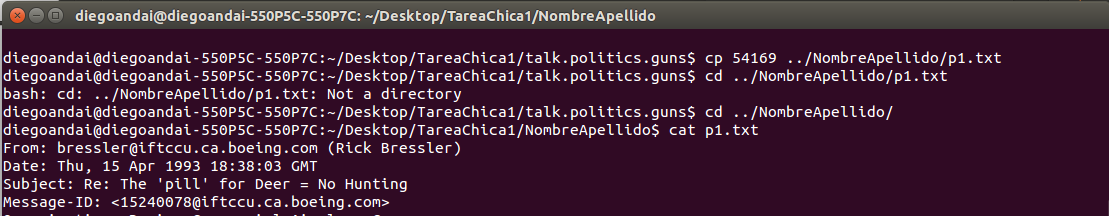
\includegraphics[scale=0.4]{tc1_paso8Redo(2).png}
\end{center}

En la imagen vemos la ejecución del comando, ademas podemos ver que los ID coinciden, tal como queríamos.

\subsection{Copiando y eliminando archivos}

Ahora se copiará un archivo del directorio sci.med al directorio NombreApellido, y luego se borrará de este mismo directorio. Para esto ocuparemos los comandos \textbf{cp} y \textbf{rm}:

\begin{lstlisting}
cp [Archivo que se va a copiar] [Adonde se va a copiar]
rm [Archivo que se va a borrar]
\end{lstlisting}

Primero encontramos algún archivo que copiar:

\begin{center}
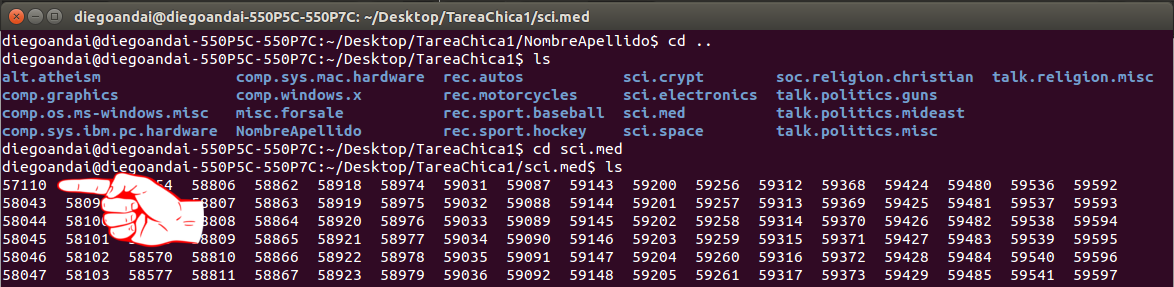
\includegraphics[scale=0.385]{tc1_14.png}
\end{center}

Copiaremos el archivo indicado (57110), por lo que necesitamos los comandos
\begin{lstlisting}
cp 57110 ../NombreApellido/
rm 57110
\end{lstlisting}

\begin{center}
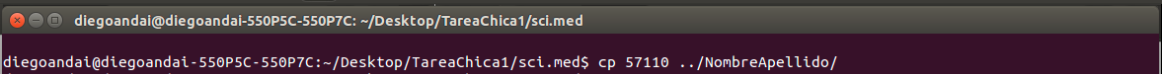
\includegraphics[scale=0.385]{tc1_paso9(1).png}
\end{center}

En la imagen anterior se implementa el primer comando, copiando el archivo a la dirección requerida

\begin{center}
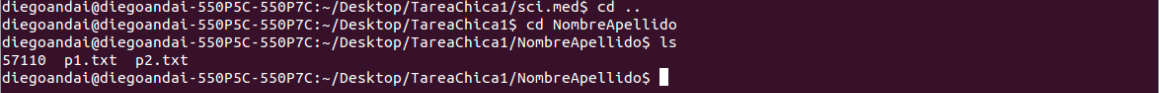
\includegraphics[scale=0.385]{tc1_paso9(2).png}
\end{center}

Revisamos el directorio NombreApellido, confirmando que el archivo 57110 fue exitósamente copiado. Ahora ocupamos el comando \textbf{rm} para borrarlo:

\begin{center}
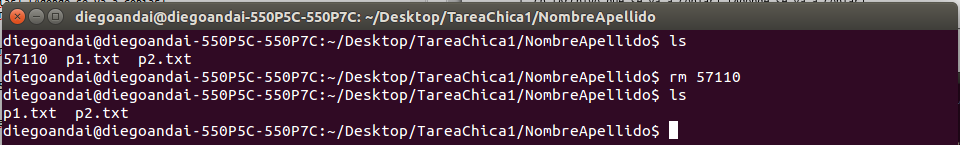
\includegraphics[scale=0.475]{tc1_paso9(3).png}
\end{center}

Confirmamos entonces que el archivo fue copiado y eliminado.

\subsection{Arreglando el error}

Al principio de la tarea, llame al directorio creado NombreApellido, pero debía llamarse DiegoAndai. Para arreglarlo ocupamos el comando \textbf{mv}:

\begin{lstlisting}
mv [nombre del directorio o archivo con el nombre original] [nuevo nombre]
\end{lstlisting}

Por lo tanto el código necesitado es:

\begin{lstlisting}
mv NombreApellido/ DiegoAndai/
\end{lstlisting}

\begin{center}

\includegraphics[scale=0.385]{tc1_error.png}
\end{center}

Error corregido!


\subsection{Finalizando la tarea}

Para finalizar, se agrega una frase de triunfo al final de p1.txt. Para esto ocuparemos el comando \textbf{echo}:

\begin{lstlisting}
echo [string]
\end{lstlisting}

El output de \textbf{echo} es un string, por lo que podemos redirigirlo hacia el archivo que se desee. Para esto se ocupa el símbolo '>>', que no reescribe todo el archivo si no que agrega al final de este, de esta forma el comando necesario es: 

\begin{lstlisting}
echo "Me encanta Computacion: Ciencia y Tecnologia del Mundo Digital! He finalizado la tarea." >> p1.txt
\end{lstlisting}

Se revisa primero que es lo que hay en el final de p1.txt:

\begin{center}

\includegraphics[scale=0.385]{tc1_paso10(1).png}
\end{center}

Implementamos el comando:

\begin{center}
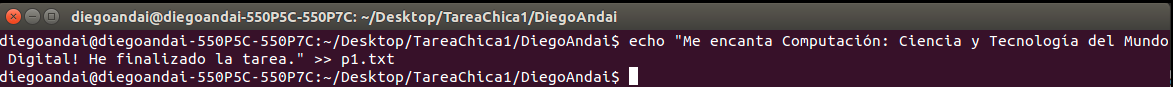
\includegraphics[scale=0.385]{tc1_paso10(2).png}
\end{center}

Por último comprobamos que los cambios sean correctos:

\begin{center}
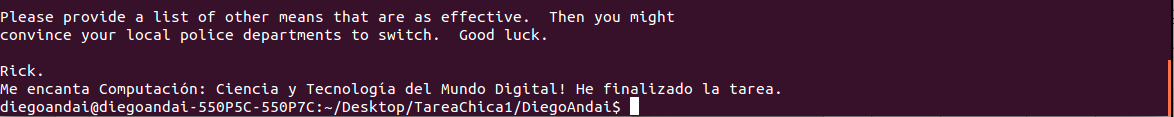
\includegraphics[scale=0.385]{tc1_paso10(3).png}
\end{center}

Y como dice la imagen, he finalizado mi tarea.

\end{document}
